\section{Introduction}
This document provides an introduction to the pythonic feedback framework as well as a manual and some examples how to write your own BCI feedbacks using this framework. It is not meant to be an introduction into Python. If you're new to Python but already have programming experience with an other language, \cite{ref:python-book} gives a very good starting point to learn Python. The documentation (especially the Library Reference) available on \cite{ref:python-onlinedoc} is essential when programming with Python.

If you don't have any programming experience, you should read \cite{ref:python-nonprogrammers-doc}.

\subsection{BCI Setup}
\index{BCI Setup}
Figure \ref{fig:setup} shows the setup of a BCI experiment. The subject is sitting in front of a monitor (if the feedback is of visual nature) and is wearing a EEG cap, collecting brain signals and submitting them to the data acquisition and signal processing units. The signal is processed and translated into Matlab code and sent to the feedback, where, depending on the feedback application, the feedback reacts on some way on the subject's EEG signals. The processed and translated EEG signal which is sent to the feedback, is called control signal\index{Control Signal}.

The experimenter has the option to control certain variables of the feedback via the GUI which also sends singals to the feedback. Those signals are called interaction signals\index{Interaction Signal}.

\begin{figure}
 \centering
 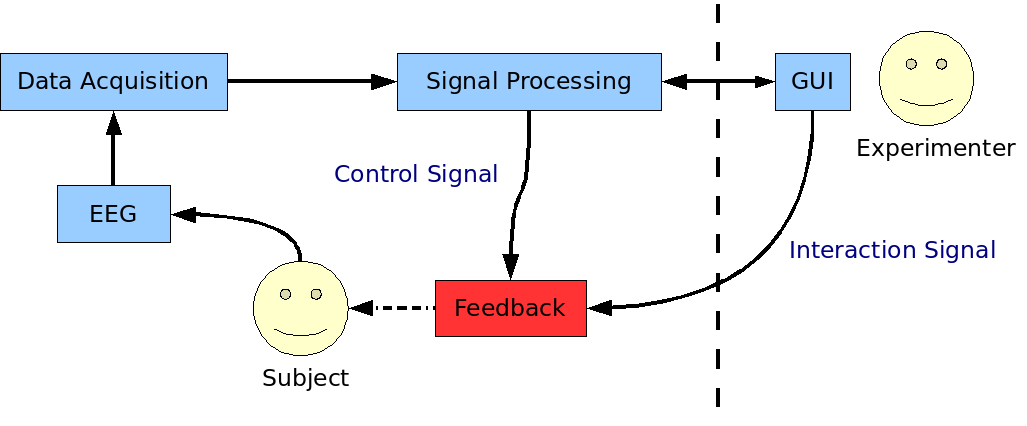
\includegraphics[width=\figwidth]{aufbau-en.png}
 % aufgabe.pdf: 595x842 pixel, 72dpi, 20.99x29.70 cm, bb=0 0 595 842
 \caption{Setup of an BCI experiment}
 \label{fig:setup}
\end{figure}

Currently everything is written in Matlab. Since many feedbacks are of a very graphic nature, may need to provide audible output and Matlab wasn't really designed for tasks like this, the BCI group wants to move away from Matlab towards Python when writing such feedbacks.

\subsection{Pythonic Feedback Framework}
The pythonic feedback framework tries to solve this task. It provides the Feedback Controller\index{Feedback Controller} which acts like a server and collects the control- and interaction signals. It also features a plugin system which makes it fairly easy to write new feedbacks in Python. Figure \ref{fig:setup2} shows the Feedback Controller in the BCI setup.
%FIXME: Wiederholung im nächsten Absatz.

\begin{figure}
 \centering
 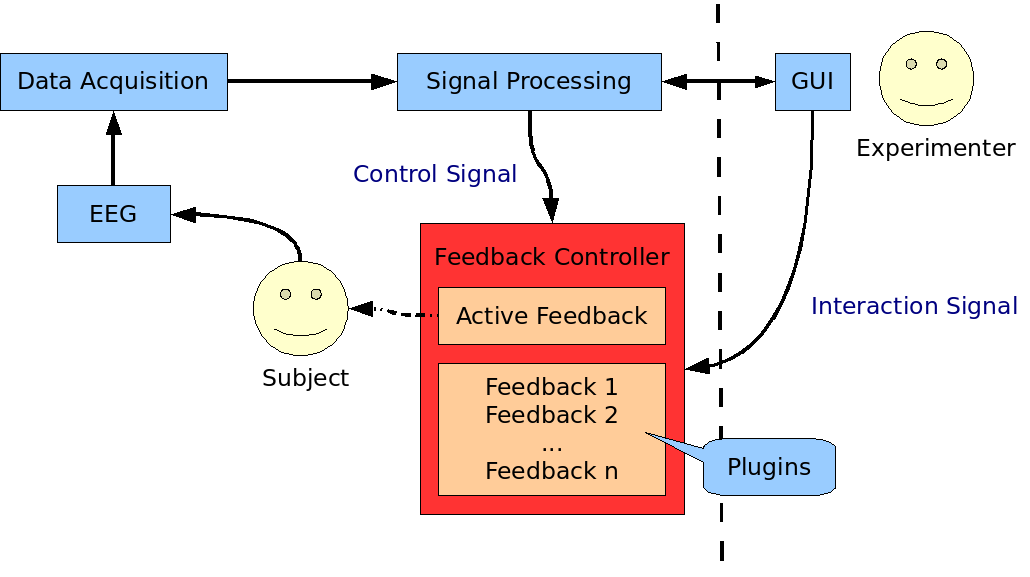
\includegraphics[width=\figwidth]{aufbau2-en.png}
 \caption{Setup of an BCI experiment with the Feedback Framework}
 \label{fig:setup2}
\end{figure}

The Feedback Controller transparently (no changes in the BCI setup are necessary) replaces the single feedback from the old setup and allows dynamic loading and un-loading of feedbacks through it's plugin system. 

\section{Introduction to the Pythonic Feedback Framework}

\subsection{Structure of the Framework}
The basic idea behind the Feedback framework is to have a Server sitting in the background collecting control- and interaction signals, translating them into Python datatypes and sending them to the currently active feedback. The server is called Feedback Controller\index{Feedback Controller}. Once started, it is fully controllable via interaction signals. You can remotely load feedbacks, start, stop and pause them via the GUI.

When receiving control signals the Feedback Controller translates the data into Python and passes the data to the currently loaded feedback.

The Feedback Controller supports a plugin system\index{Plugin-System} which makes it very easy to create new feedbacks. Basicly all you have to do to create a new feedback is to subclass the Feedback base class and implement the functions as needed or create your own ones.

\subsection{The Feedback Base Class}
The Feedback\index{Feedback} base class is the interface to the Feedback Controller's plug-in system. By subclassing the Feedback class and putting it somewhere into the Feedbacks directory\index{Feedbacks Directory} your feedback is already a valid and ready-to-use (although quite useless at this moment) feedback, available to the Feedback Controller.

The mode of operation of the feedbacks is event driven. Whenever the Feedback Controller receives a signal, it translates and analyzes it and calls the appropriate method of the feedback to notify it. When writing your own feedback, all you have to do is to implement some or all methods of the Feedback base class to react on those signals as needed.

The following methods are supported by the Feedback base class:
\begin{description}
\item[on\_init(self)]\index{Feedback!on\_init} This method is called by the Feedback Controller after the feedback has been successfully loaded. Since the initialization of the feedback is triggered by an interaction signal, \lstinline+on_interaction_event+ is called right after \lstinline+on_init+ returned.
\item[on\_interaction\_event(self, data)]\index{Feedback!on\_interaction\_event} This method is called when the Feedback Controller received an interaction signal. data contains all the variables sent by the GUI. You don't have to use the data from here directly, see section \ref{sec:is} for details.
\item[on\_control\_event(self, data)]\index{Feedback!on\_control\_event} This method is called by the Feedback Controller after the Feedback Controller received a control signal. data contains the tuple containing the processed and translated EEG data. You don't have to use this variable, see section \ref{sec:cs} for details.
\item[on\_play(self)]\index{Feedback!on\_play} If the Feedback Controller detects the Play\index{Interaction Signal!Play} command in an interaction signal, it calls this method just before it calls \lstinline+on_interaction_event+.
\item[on\_pause(self)]\index{Feedback!on\_pause} If the Feedback Controller detects the Pause\index{Interaction Signal!Pause} command in an interaction signal, it calls this method just before it calls \lstinline+on_interaction_event+.
\item[on\_quit(self)]\index{Feedback!on\_quit} If the Feedback Controller detects the Stop\index{Interaction Signal!Stop} command in an interaction signal, it calls this method just before it calls \lstinline+on_interaction_event+.
\item[send\_parallel(self, data)]\index{Feedback!send\_parallel} This is the only method of the Feedback base class which actually provides functionality. You should not overwrite this method if you don't want to replace the underlying code. Use this method to send a byte to the parallel port of the machine running the feedback.
\end{description}
\lstinline+on_play+, \lstinline+on_pause+ and \lstinline+on_quit+ are a convenient methods which are always called before \lstinline+on_interaction_event+. You don't have to use them but then you will almost certainly have to inspect every interaction signal to check whether it contains the Start, Pause or Stop trigger if you want to react on them.

\subsection{Interaction Signals}\label{sec:is}
\index{Interaction Signal}
Everytime the Feedback Controller receives a valid interaction signal from the GUI, it translates it and calls the \lstinline+on_interaction_event+ method of the currently running feedback. We can distinguish between five different types of interaction signals:
\begin{description}
\item[Send] \index{Interaction Signal!Send}With this signal the GUI sends various variable-value pairs to the feedback.
\item[Send+Init] \index{Interaction Signal!Send+Init}Like the Send signal plus the command to initialize the feedback.
\item[Start] \index{Interaction Signal!Start}This signal tells the feedback to start its main routine (e.g. the trials).
\item[Pause] \index{Interaction Signal!Pause}Tells the feedback to pause the run.
\item[Stop] \index{Interaction Signal!Stop}Tells the feedback to quit.
\end{description}
If the Feedback Controller recognizes a generic interaction signal (Send) it just calls \lstinline+on_interaction_event+ of the feedback. If it additionally recognizes an Init, Start, Pause or Stop command in the signal, it also calls the appropriate \lstinline+on_+-method of the feedback. In case of Init, it calls \lstinline+on_init+ before \lstinline+on_interaction_event+, in every other case after. Table \ref{tab:is-triggers} shows the ordering of the method calls of the feedback triggered by the different interaction signals.
\begin{table}
\centering
\begin{tabular}{l||l}
\textbf{GUI sends} & \textbf{Feedback receives} \\
\hline\hline
Send & \lstinline+on_interaction_event(self, data)+\\
\hline
Send+Init & \lstinline+on_quit(self)+ (old feedback)\\ 
          & \lstinline+on_init(self)+ \\ 
          & \lstinline+on_interaction_event(self, data)+ \\ 
\hline
Start & \lstinline+on_interaction_event(self, data)+ \\ 
      & \lstinline+on_play(self)+ \\ 
\hline
Pause & \lstinline+on_interaction_event(self, data)+ \\ 
      & \lstinline+on_pause(self)+ \\ 
\hline
Stop & \lstinline+on_interaction_event(self, data)+ \\ 
     & \lstinline+on_quit(self)+
\end{tabular}
\caption{Overview of the method calls triggered by the different types of interaction signals.}\label{tab:is-triggers}
\end{table}

The Feedback controller also analyzes the data in the interaction signal, extracts the variables and it's values and puts them into the currently running feedback. See \ref{sec:working-with-cs-is} for details.

\subsection{Details About the Matlab-Python Translation}
The unpacked control- and interaction signal is in fact code which is directly interpretable by Matlab. The control signal contains just a tuple of numbers representing the processed EEG signal, the interaction signal contains Matlab variable-assignments. Since the Matlab syntax and it's data types are not Python compatible, it is necessary to translate the variable names and Matlab's datatypes into Python.

\paragraph{Translation of Variablenames}
The translation of Matlab's variable names is straightforward. The only important aspect is that if the Feedback Controller detects dots in the variable names it truncates the name after the last dot and takes the result as variable name.

If for example the Feedback Controller receives a variable \verb+feedback_opt(1).type+, the resulting variable name in the feedback will be \lstinline+_type+ (note the underscore prefix, see section \ref{sec:working-with-cs-is} for details). If the Feedback Controller receives a variable name without a dot, the whole name will be taken on if possible.

\paragraph{Translation of Datatypes}
\index{UdpDecoder}
Matlab supports many data types which have no equivalent in Python while it also shares a subset of types which have a equivalent in Python. Fortunately the Feedback Controller does not have to support all available types available in Matlab (although it would be possible). Only the most common ones like strings, integers, floats and lists are needed to communicate with the feedbacks. All of them are currently recognized. If the Feedback Controller receives an unknown type it will print out a warning and move on. If needed the Feedback Controller can be enhanced to recognize more types. The relevant method is \lstinline+__parse_type+\index{UdpDecoder!\_\_parse\_type} of the UdpDecoder class.


\subsection{Control Signals}\label{sec:cs}
\index{Control Signal}
Whenever the Feedback controller receives a control signal, it translates it, extracts the data (a tuple containing a few numbers), puts it in the currently running feedback (see \ref{sec:working-with-cs-is} for details) and calls the feedback's \lstinline+on_control_event(self, data)+ method.

\section{Writing Your Own Feedbacks}
\label{ref:writing-your-own-feedbacks}
The Feedbacks/Tutorial directory contains a few example feedbacks which will hopefully help you to understand how to develop your own ones. This section will explain them.

\subsection{Naming Convention for the Module- and Class Name}\label{sec:namingconvention}
\index{Feedback!Naming Convention}
\index{Plugin-System}
In order to make your Feedback available to the Feedback Controller's plugin system, your feedback has to follow a certain naming convention. The rules are:
\begin{enumerate}
\item \textit{The feedback has to be located somewhere in the Feedbacks directory.} It is possible to place it in an arbitrary deep subdirectory inside of the Feedbacks directory. There are no restrictions on the subdirectories names as long as they represent valid Python packages.
\item \textit{The feedback's class name must match it's module name.} If the class name of your feedback is \lstinline+FooBar+ then it has to be written in the file \verb+FooBar.py+.
\end{enumerate}


When the experimenter wants to load a certain feedback, he sends a Send+Init signal which contains at least the assignment of the \lstinline+type+ variable. The variable holds a string which is interpreted in the following way: 
\begin{itemize}
\item If the string contains no dots (the "." character), the string is interpreted as the module \textit{and} class name of the feedback.
\item If the string contains one or more dots, the string is split up and the last element represents the module/class name and the element(s) before the last element the package name.
\end{itemize}

\paragraph{Examples:}
\begin{itemize}
\item If the Send+Init signal contains \lstinline+type = Foo.baR.Baz+, the Feedback controller tries to load the Class \lstinline+Baz+ in the module \verb+Baz+ (the file \verb+Baz.py+) in the Directory \verb+Feedbacks/Foo/baR+.
\item If the Send+Init signal just contains \lstinline+type = MyFeedback+, the Feedback Controller searches for the class \lstinline+MyFeedback+ in the module \verb+MyFeedback+ located directly in the \verb+Feedbacks+ directory.
\end{itemize}


\subsection{Subclassing the Feedback Class}
Following the naming conventions of section \ref{sec:namingconvention} ensures that the Feedback Controller \textit{finds} the plugin. In order to make it working properly as a valid plugin of the Feedback Controller, the feedback has to be a subclass of the \lstinline+Feedback+ base class.

Listing \ref{list:lesson01} shows a fully working Feedback without any functionality other than printing the feedback has been successfully loaded and quit. The lines 1-3 are the important ones in this lesson: You have to import the Feedback class from the Feedback package and subclass your Feedback (Lesson01 in this case) from it. You don't have to override the on\_init and on\_quit methods to make the feedback working if you would replace the lines 5-9 with a simple \lstinline+pass+ statement, the feedback would still be perfectly running without any functionality.

\begin{lstlisting}[caption=Trivial Feedback, label={list:lesson01}]
from Feedback import Feedback

class Lesson01(Feedback):
    
    def on_init(self):
        print "Feedback successfully loaded."
    
    def on_quit(self):
        print "Feedback quit."
\end{lstlisting}

\paragraph{Overwriting \lstinline+Feedback.__init__+} Since the \lstinline+__init__+ method of the Feedback base class is already implemented (it sets up the feedbacks logger and opens the parallel port), you should not overwrite it blindly. If you want to overwrite it, make sure to call the base class' \lstinline+__init__+ method before anything else in this method. Listing \ref{list:lesson01b} shows an example. The second parameter is a handle to the parallel port, the third parameter of the \lstinline+__init__+ method changes the prefix the feedback uses for variables which are automaticly set and updated by the feedback controller (see \ref{sec:working-with-cs-is} for details). The parameter is optional and defaults to the underscore character if omitted.

\begin{lstlisting}[caption=Trivial Feedback with \lstinline+__init__+ overwritten, label={list:lesson01b}]
from Feedback import Feedback

class Lesson01b(Feedback):
    
    def __init__(self, pp):
        Feedback.__init__(self, pp, "foo-")
        # Your own stuff goes here
    
    def on_init(self):
        print "Feedback successfully loaded."
    
    def on_quit(self):
        print "Feedback quit."
\end{lstlisting}

Since Feedback's \lstinline+on_init+ is guaranteed to be the next method called after \lstinline+__init__+ it should not be necessary to overwrite \lstinline+__init__+ in most cases. You should use \lstinline+on_init+ instead.

\subsection{Reacting on Play, Pause and Stop/Writing a Threaded Main Loop}
Listing \ref{list:lesson02} shows a very simple feedback which is already able to react on Play, Pause and Stop interaction signals. It starts it's main loop in a new thread which does nothing more than incrementing a number and sleeping for a half second. Although very simple, this example already contains many important aspects of real life feedbacks.
%, since you almost certainly want to have some kind of main loop running in a separate thread, which is pausable and stopable via interaction events.

\paragraph{\lstinline+on_play+ runs in a different thread} It is very important to know that \lstinline+on_play+ runs in a different thread than all the other Feedback methods. This is important since in most cases the \lstinline+on_play+ method will execute for a potentially long time (like several minutes). In order to allow the Feedback Controller to call other methods of the Feedbacks in the meantime, it is necessary to let this method run in a different thread than the other ones.

\paragraph{How to make sure \lstinline+on_quit+ only returns when the main loop is finished?} Since the main loop of the feedback will run in a different thread than the rest of the Feedback's methods, you have to make sure that the \lstinline+on_quit+ method does not return until the other thread is killed. In order to achieve that you should set a variable (in this example \lstinline+quitting+) which will cause the main loop to exit and wait until another variable (\lstinline+quit+) has been set by the main loop when it exited. This can be done by a simple loop which does nothing until the \lstinline+quit+ variable has been set by the main loop (busy waiting).

\begin{lstlisting}[caption=A more realistic example., label={list:lesson02}]
# Lesson02 
#  - Starting a main loop in a thread when the feedback gets the start signal
#  - Pausing and unpausing it
#  - Quitting the main loop

from Feedback import Feedback

import time

class Lesson02(Feedback):
    
    def on_init(self):
        print "Feedback successfully loaded."
        self.quitting, self.quit = False, False
        self.pause = False
    
    def on_quit(self):
        self.quitting = True
        # Make sure we don't return on_quit until the main_loop (which runs in
        # a different thread!) quit.
        print "Waiting for main loop to quit."
        while not self.quit:
            pass
        # Now the main loop quit and we can safely return

    def on_play(self):
        # Start the main loop. Note that on_play runs in a different thread than
        # all the other Feedback methods, and so does the main loop.
        self.quitting, self.quit = False, False
        self.main_loop()
        
    def on_pause(self):
        self.pause = not self.pause
        
    def main_loop(self):
        i = 0
        while 1:
            time.sleep(0.5)
            if self.pause:
                print "Feedback Paused."
                continue
            elif self.quitting:
                print "Leaving main loop."
                break
            i = i+1
            print "Iteration Number %i" % i
        
        print "Left main loop."
        self.quit = True
\end{lstlisting}

\subsection{Working With Data Sent by Control- and Interaction Signals}
\label{sec:working-with-cs-is}
The Feedback Controller provides a very convenient way to access the data sent by the control- and interaction signals. Listing \ref{list:lesson03} shows a snippet of Lesson03, which is a variant of Lesson02 as shown in Listing \ref{list:lesson02} with a modified main loop. The listing demonstrates how to access the data sent by the control- and interaction signal.

\paragraph{Control Signal} The data sent by the control signal is stored automaticly in the \lstinline+_data+ variable of your feedback. Everytime the Feedback Controller receives a control signal it overwrites the \lstinline+_data+ variable with the new value.

\paragraph{Interaction Signal} The variable assignments sent via the interaction signal are translated into Python and also stored as variables in your feedback. If the interaction signal contains \verb+foo='some string',bar=123,baz=74.11+ then your feedback automaticly provides the variables \lstinline+_foo+, \lstinline+_bar+ and \lstinline+_baz+ with the corresponding values.

\begin{lstlisting}[caption=Accessing control- and interaction data., label={list:lesson03}]
    def main_loop(self):
        i = 0
        while 1:
            time.sleep(0.5)
            if self.pause:
                print "Feedback Paused."
                continue
            elif self.quitting:
                print "Leaving main loop."
                break
            print self._data
            print self._type
            
        print "Left main loop."
        self.quit = True
\end{lstlisting}

\paragraph{The escape character} \index{Escape Character}In order to avoid pollution of the namespace of your feedback, all the variables which are created and updated automaticly by the Feedback Controller are prefixed. By default the prefix is a single underscore character ("\_"), you can change the prefix by calling the \lstinline+Feedback.__init__(self, prefix="_")+ method. As you can see the prefix parameter is optional an by default the undersore. Listing \ref{list:lesson01b} shows a variant where the prefix is \verb+foo-+. In that case the variables in the above examples would be \lstinline+foo-data+, \lstinline+foo-foo+, \lstinline+foo-bar+ and \lstinline+foo-baz+.

\subsection{Reacting on Control- and Interaction Events}
Since the Feedback Controller already stores the data sent by the interaction- and control signals in the feedback, it should not be necessary to directly react on control- or interaction events in most cases (Please consider the hints about coding style in section \ref{ref:codingstyle-is}). However, in some cases you might want to do something whenever the feedback receives such a signal. In this case you have to overwrite \lstinline+on_interaction_event+ respectively \lstinline+on_control_event+. Both methods have the \lstinline+data+ variable which holds the processed and translated contents of the signal. At the time the methods are called those data is already present as attributes in the feedback.

\begin{lstlisting}[caption=Reacting on control- and interaction events., label={list:lesson04}]
from Feedback import Feedback

class Lesson04(Feedback):
    
    def on_init(self):
        self.myVariable = None
        self.eegTuple = None
    
    def on_interaction_event(self, data):
        # this one is equivalent to:
        # self.myVariable = self._someVariable
        self.myVariable = data.get("someVariable")
        print self.myVariable
        
    def on_control_event(self, data):
        # this one is equivalent to:
        # self.eegTuple = self._data
        self.eegTuple = data
        print self.eegTuple
\end{lstlisting}

Listing \ref{list:lesson04} shows a trivial example how to react on interaction- and control events. 

\subsection{Sending Markers to the Parallel Port}
Most feedbacks need to send so called markers\index{Markers} to the parallel port on various events. For this task the Feedback base class provides the \lstinline+send_parallel(self, data, reset=True)+\index{Feedback!send\_parallel} method, which sends the given data to the parallel port if possible.

Unlike the other methods of the Feedback base class you don't need to overwrite this method to do something usefull. The method is already implemented in the Feedback base class.

The \lstinline+send_parallel+ method will send the given byte to the parallel port and reset the port again to zero after 10ms. Listing \ref{list:lesson05} shows the example feedback Lesson05.

\begin{lstlisting}[caption=Sending markers., label={list:lesson05}]
from Feedback import Feedback

class Lesson05(Feedback):
    
    def on_init(self):
        self.send_parallel(0x1)
    
    def on_play(self):
        self.send_parallel(0x2)
    
    def on_pause(self):
        self.send_parallel(0x4)
    
    def on_quit(self):
        self.send_parallel(0x8)
\end{lstlisting}

Read section \ref{sec:pp-linux} if you have problems acessing the parallel port under Linux.

\subsection{Using the Framework's Logging Facility}
\index{Logging}\index{Feedback!logger}
The Feedback base class already has a logger build in, available through the \lstinline+self.logger+ variable. Listing \ref{list:lesson06} shows Lesson06, a modified version of Lesson01 as shown in \ref{list:lesson01}. Instead of a simple \lstinline+print+, this version uses the logger which can be silenced at a central point in the Feedback Controller so you don't have to comment in and -out all the print lines as you would do without using a logger.

\begin{lstlisting}[caption=Using the Feedback's logger., label={list:lesson06}]
from Feedback import Feedback

class Lesson06(Feedback):
    
    def on_init(self):
        self.logger.debug("Feedback successfully loaded.")
    
    def on_quit(self):
        self.logger.debug("Feedback quit.")
\end{lstlisting}

\paragraph{Configuring the Logger} The framework's logging facility is configurable through command line parameters:
\begin{description}
\item[--loglevel=LOGLEVEL] Controls which messages appear on the console and which are suppressed. Possible values are in ascending order: notset, debug, info, warning, error and critical, the default loglevel is warning. Setting the loglevel to error means every message with a level error and higher will be printed out to the console, while the messages with a lower level than error are suppressed.

This option controls the loglevel of the Feedbacks and the Feedback Controller. It's use is equivalent of setting both levels (see below) separately to the same level.
\item[--fb-loglevel=LOGLEVEL] Sets the loglevel for the Feedback, default is warning.
\item[--fc-loglevel=LOGLEVEL] Sets the loglevel for the Framework, default is warning.
\end{description}
Note that you can assign a different loglevels to the feedback and the framework. This is very useful if you want to use lower loglevels for your feedback but are not interested in the low level logmessages of the feedback controller.

Since the loglevel option sets both levels: for the Feedbacks and the Feedback Controller, it is possible to set conflicting loglevels. If you set conflicting loglevels, the lowest of the desired loglevels will be taken. 

\paragraph{Example: } Setting \verb+--loglevel=info --fb-loglevel=debug --fc-loglevel=warning+ will set the loglevel for the Feedback Controller to \verb+info+ since it is the smallest of the two conflicting values \verb+info+ and \verb+warning+. The loglevel for the Feedbacks will be set to \verb+debug+ since \verb+debug+ is lower than \verb+info+.

\subsection{FeedbackCursorArrow -- a Complete Example}
The above sections only discussed single aspects of writing feedbacks. There also exists a complete example feedback called FeedbackCursorArrow\index{CursorArrow Feedback}. It is a complete rewrite of the Matlab feedback \lstinline+Feedback_cursor_arrow+. The feedback is a game where an arrow is randomly shown pointing at one of two different directions and where the subject has to try to move a cursor to the correct direction into the target zone in a short period of time.

The feedback is located in the Feedbacks directory and gives you an example how a feedback written in Python, using the Framework and Pygame could look like.

\section{Notes}
\subsection{Packages the Framework Depends on}\
In order to get the framework running you have to install the following packages:
\begin{description}
\item[Python] The framework needs this package to execute. The version under which the framework was developed is 2.4.
\item[pyParallel] \index{pyParallel}Used by the framework to utilize the machine's parallel port. You can download it from here \cite{ref:pyparallel} or on Debian based distributions get it by installing the package python-parallel.
\item[pyGame] Download it from here \cite{ref:pygame}, the according Debian package is called: python-pygame
\end{description}

\subsection{Using Threads in Your Feedback}
\index{Threads}
If you for some reason have to use threads in your feedback, you should take special care to kill them before the feedback returns it's \verb+on_quit+ method. Please keep in mind, that by default the Feedbacks \lstinline+on_play+ method already runs in a different thread than all the other methods of the Feedback (and so do all the methods which are called by this method).

Python supports two ways of using threads in your application. The first one comes from the thread-module\index{Threads!thread module} and provides very low-level primitives for working with multiple threads \cite{ref:pydoc-thread}. The \lstinline+start_new_thread(function, args[, kwargs])+ method provides a painless way to start a method in a new thread. Unfortunately it does not return a handle to the thread and you have no way to control it directly.

The second way is to use Python's threading module \index{Threads!threading module}. It provides higher-level interfaces on top of the low-level thread module \cite{ref:pydoc-threading}. Among others, it provides the Thread class which provides important methods like \lstinline+start+, \lstinline+join+ and \lstinline+isAlive+. The \lstinline+join+ method is particularly important if you want to make sure that the \lstinline+on_quit+ method of your feedback does not return before all the threads of the feedback have quit. Listing \ref{list:fca-quit} shows an example, where the \lstinline+on_quit+ method checks via \lstinline+isAlive+ if the thread is alive and waits until the thread has quit before calling \lstinline+pygame.quit()+ and returning to the Feedback Controller.

\begin{lstlisting}[caption=on\_quit method of the CursorArrow-Feedback., label={list:fca-quit}]
    def on_quit(self):
        self.quit = True
        if self.someThread.isAlive():
            self.someThread.join()
        pygame.quit()
\end{lstlisting}

\subsection{Pygame and Threads}
When writing a graphical feedback in Python using Pygame\index{Pygame}, you will almost certainly want to use pygame.time.Clock.tick(FPS)\index{Pygame!time.Clock.tick} to limit the framerate your feedback is running. Python currently does not utilize more than one CPU and just emulates threads by running each thread for a small amount of time sequentially. For a detailed explanation about Python's way of handling threads and a nice introduction into threads in general see \cite{ref:pythreads}. 

Under some circumstances Pygame's clock.tick() implementation might use busy waiting and will therefore not put the thread to sleep to share the processor with other threads. Since most reasonable non-trivial feedbacks will at least use one thread for their main loops, this could lead to a situation where the framework's network threads starve and aren't able to provide new control- and interaction signals.

A workaround for this problem is to forcefully put the thread into sleep for a small amount of time before limiting the framerate via Clock.tick(). So instead of the intuitive variant in listing \ref{list:fps}

\begin{lstlisting}[caption=Limiting the framerate the intuitive (but wrong) way., label={list:fps}]
self.clock.tick(self.FPS)
\end{lstlisting}

you should wait for a small amount of time to put the thread into the sleeping state to share the CPU with the other threads. Listing \ref{list:fps2} shows an example.

\begin{lstlisting}[caption=A working alternative., label={list:fps2}]
pygame.time.wait(10)
self.clock.tick(self.FPS)
\end{lstlisting}

wait(10) will sleep the current thread for 10 milliseconds and share the processor with other threads. Since \lstinline+tick()+ remembers the time it was called the last time, calling \lstinline+wait(n)+ will have no negative effects as long as the sum of the time $n$ and the time needed for one loop of the main loop is not bigger than the reciprocal of the desired framerate.

\subsection{Pygame and Threads II}
Another important aspect of threading with Pygame comes with a limitation of pygame: The \lstinline+pygame.init()+ and the polling of Pygame's event queue have to take place in Python's main thread! Otherwise on some operating systems the whole application will not respond correctly to the operating system an might appear to be hanging.

The Feedback's \lstinline+on_play+ method already runs in Python's main thread for this very reason. All you have to take care of is to initialize pygame and poll pygame's event queue in this method (or in one of the methods \lstinline+on_play+ calls).

\subsection{Polling Pygame's Event Queue}
This important point is somewhat hidden in pygame's online documentation \cite{ref:pygame-events}: 
\begin{quotation}
"Your program must take steps to keep the event queue from overflowing. If the program is not clearing or getting all events off the queue at regular intervals, it can overflow. When the queue overflows an exception is thrown."
\end{quotation}

This means that you must poll pygame's event queue once per frame(!) even if you don't use the event queue.

The example \lstinline+FeedbackCursorArrow+ provides a method \lstinline+process_pygame_events+ which can serve as an example. It polls the event queue to react on changes of the window dimensions.

If you don't use pygame's event queue, you still have to poll the queue so pygame can process the events internally, you can achieve this by calling \lstinline+pygame.event.pump()+ once per frame

\subsection{Good Coding Style Regarding the Interaction Signal}
\label{ref:codingstyle-is}
Allthough the Feedback Controller automaticly creates and updates variables in your feedback on interaction signals, you should consider having a central point where you connect the variable names from the interaction signal with the counterparts of your feedbacks. For example if the GUI sends the \verb+foo+ variable and your feedback uses the \lstinline+_foo+ provided by the Feedback Controller many times on different places in the code. Imagine the variable name is changed in the GUI from \verb+foo+ to \verb+bar+, now you would have to search all over the code and change all occurrences of \lstinline+_foo+ to \lstinline+_bar+. This can be done semi automaticly with the right tools but is a potentially dangerous action (imagine you already had a variable called \lstinline+_foo+).

A clean solution would be to utilize the \lstinline+on_interaction_event+ method of your feedback to translate the external variable names to your local ones. This way you would have one central point where you would have to care about each variable from the interaction signal exactly once.

\subsection{Using the Parallel Port Under Linux}
\label{sec:pp-linux}
\index{Parallel Port}
On our Linux systems running Debian/Etch we were not able to use the parallel port by default. The problem was the lp kernel module which occupies the parallel port and insufficient user permissions to use the parallel port. The following commands in listing \ref{list:pp} will unload the lp kernel module and make the parallel port writable for everyone.
\begin{lstlisting}[language=bash, caption=Making the parallel port available on Debian/Etch, label={list:pp}]
user@box$ sudo modprobe -r lp
user@box$ sudo chmod 666 /dev/parport0
\end{lstlisting}
This has to be done everytime the machine on which the framework is running is rebooted.

